\documentclass[paper=a4,notitlepage,parskip=half,plainheadsepline]{scrartcl}
 
\usepackage{scrlayer-scrpage} 
\usepackage{ngerman}
\usepackage{graphicx}
\usepackage{float}
\usepackage[T1]{fontenc}
\usepackage[utf8]{inputenc}
\usepackage{pifont}
\usepackage{amsmath}
\usepackage{textcomp}
\usepackage[german]{varioref}
\usepackage[text={6.8in,9.6in},top=0.7in,centering]{geometry}
\usepackage{datetime2}
\usepackage{array,multirow,tabularx}
\usepackage{listingsutf8}
\usepackage[table,svgnames,dvipsnames]{xcolor}
\usepackage[most,breakable,skins,listingsutf8]{tcolorbox}
%\tcbuselibrary{listingsutf8}
\usepackage[color=blue!90,scale=0.8,placement=bottom,vshift=1.2cm]{background}
\usepackage{array}
\usepackage{physics}
\usepackage{tikz}
\usepackage{pgfplots}
\usepgflibrary{shapes.symbols}
\usetikzlibrary{arrows}
\pgfplotsset{compat=1.16}

%%%%%%%%%%%%%%%%%%%%%%%%%%%%%%%%%%%%%%%%%%          Aufgabe oder Loesung 
\newif\ifloesung
%\loesungtrue
\loesungfalse
%%%%%%%%%%%%%%%%%%%%%%%%%%%%%%%%%%%%%%%%%%%%%%%%%%%%%%%%%%%%%%%%%%%%%%%%%

%\backgroundsetup{contents={Version vom \today}}
\backgroundsetup{contents={Version vom \today}}
%\pagestyle{empty}

\pagestyle{scrheadings}
\clearpairofpagestyles
\ihead{Fachinformatiker Anwendungsentwickler / Dualer Studiengang}
\chead{}
\ohead{C/Python Simulation}
\ifoot{Frank Zimmermann}
\cfoot{SVLFG}
\ofoot{}
\ofoot{\pagemark}

\graphicspath{{./jpg/}}
\DeclareGraphicsExtensions{.jpg,.eps,.png}
%\usepackage{courier}


%\newcommand\bashprompt{\textcolor{cyan}{\small\ttfamily\bfseries{bob@remotehost{\textcolor{black}:}\textcolor{cyan!60}{\url{~}}{\textcolor{black}\$ }}}}
\newcommand\bashprompt{\textcolor{red!25!white}{\small\ttfamily\bfseries bash\$> }}
\newcommand\noprompt{\hspace{0.6cm}}
\newcommand{\startBash}{\gdef\myprompt{\bashprompt}}
\newcommand{\startNone}{\gdef\myprompt{\noprompt}}

\newcommand{\mingw}{\textsl{MinGW}}
\newcommand{\bash}{\emph{bash}}
\newcommand{\msys}{\textsl{MSYS}}
\newcommand{\git}{\emph{Git}}
\newcommand{\gcc}{\emph{gcc}}
\newcommand{\listingsfont}{\ttfamily}

\RedeclareSectionCommand[
  beforeskip=-1\baselineskip,
  afterskip=.5\baselineskip]{section}
\RedeclareSectionCommand[
  beforeskip=-.75\baselineskip,
  afterskip=.5\baselineskip]{subsection}
\RedeclareSectionCommand[
  beforeskip=-.5\baselineskip,
  afterskip=.25\baselineskip]{subsubsection}
\RedeclareSectionCommand[
  beforeskip=.5\baselineskip,
  afterskip=-1em]{paragraph}
\RedeclareSectionCommand[
  beforeskip=-.5\baselineskip,
  afterskip=-1em]{subparagraph}

% Wenn pdflatex benutzt wird sollen die 
% installierten! frutiger-Fonts verwendet werden
% Ansonsten die TeX-eigenen cmbright
\ifpdfoutput %
{%
\usepackage[scaled=0.90]{frutiger}
\renewcommand\familydefault{\sfdefault}
%\DeclareFixedFont\ott{T1}{phv}{mc}{n}{10pt
}%
{%
\usepackage{cmbright}
}%

\newfont{\lf}{svlfg scaled 2000}%
\newcolumntype{P}[1]{>{\centering\arraybackslash}p{#1}}

\ifloesung
\newtcbinputlisting[auto counter,list inside=lol,list type={lstlisting}]{\mylisting}[4][]{%
  toptitle=2mm,
  bottomtitle=2mm,listing only,
  colback=lightgray,
  %colback=yellow!10,
  listing file={#3},
  listing options={language=#4,
  aboveskip=5pt,
  belowskip=5pt,
  columns=flexible,
  keywordstyle=\color{blue},
  basicstyle=\footnotesize\listingsfont},
  colback=white,
  %colframe=gray!75!black,
  colframe=yellow!50!black,
  listing only,
  fonttitle=\bfseries,
  breakable,
  %title={Soubor \thetcbcounter: #2},
  title=Musterlösung für \texttt{#3},
  #1
}
\fi

\begin{document}
\tcbset{enhanced,colback=green!5!white, boxrule=0.5pt, colframe=green!35!black,fonttitle=\bfseries\Large}
        % \begin{tcolorbox}[drop lifted shadow]
        % This is a tcolorbox.
        % \end{tcolorbox}\par\bigskip
        \begin{tcolorbox}[toptitle=3mm,bottomtitle=3mm,title=\centering{{\lf J}\hfil FI Anwendungsentwicklung / Duales Studium\hfil {\lf J}},
          drop lifted shadow=gray]
        \centering{\vspace{0.5cm}\LARGE Programmierübung %
        \ifloesung (mit Musterlösung)\fi}\\[0.3cm]
        \centering{C/Python--Programmierung / Simulation / Nash--Gleichgewichte}\\\vspace{0.5cm}
        \end{tcolorbox}

\section{Szenario I}
Wie heißt es so schön: Die Märkte sind kompliziert!

Aber nicht immer sind die Märkte so kompliziert, dass man sie nicht berechnen kann.

Folgendes Szenario ist vorhanden:

Ein Produkt wird nur von 2 Unternehmen hergestellt (ein sogenanntes Angebots--Oligopol/Duopol). Beide Unternehmen wollen Gewinne mit diesem Produkt erzielen und damit am Markt überleben. Beide Unternehmen wissen, dass ein hartnäckiger Preiskampf ein Unternehmen in die Insolvenz treiben würde. Da aber genug Nachfrage herrscht, könnten eigentlich beide Firmen gleichzeitig Gewinne machen und dabei überleben.

Durch Meinungsumfragen (gab es umsonst vom {Zu\-lieferer}) wissen beide Firmen, wie hoch die Nachfrage für ihre Produkte in Abhängigkeit ihrer Preise ($p_1$,$p_2$) ist.
Die Herstellungskosten pro Produkt sind für beide Unternehmen gleich ($c=3/2$) und müssen natürlich zur Gewinnermittlung vom erzielten Produkt--Preis abgezogen werden. 

Beide Firmen haben einen langen Vorlauf für ihre Werbekampagne (Kosten werden ebenfalls vom {Zu\-lieferer} übernommen). Sie können ihre Preise nur \emph{einmal} zu Beginn der Markteinführung festlegen und daher sollten sie gut gewählt werden.
Sind sie zu gering oder zu hoch, kann sich die Nachfrage ungünstig ändern, das dann zu einer Verringerung der Einnahmen führen würde.

\section{Aufgabe}
Ihre Aufgabe ist es, für ihr Unternehmen (sagen wir Unternehmen~1) den Preis so zu kalkulieren, dass das Unternehmen~1 einen maximalen Gewinn erziehlen kann.

Wichtigste Information ist daher die Marktanalyse, die angibt, wieviele Kaufabsichten bei einem bestimmten Preis $p_1=p_2=p$ für jeweils ein Unternehmen zu erwarten sind (Nachfrage--Funktion/Demand Function: $D_1(p_1,p_2)$ bzw. $D_2(p_1,p_2)$):

\begin{equation}
D_1 = 5 - p \qquad\text{bzw.}\qquad D_2 = 5 - p \qquad\text{mit}\quad p=p_1=p_2 
\end{equation}

Wie man sieht, ist das Problem symmetrisch, was die Lösung doch sehr vereinfacht, da der maximale Preis automatisch für beide Unternehmen gilt.
D.h., da die Nachfragefunktion auch für das Unternehmen~2 gilt, wird auch Unternehmen~2 den gleichen Preis wie Unternehmen~1 verlangen, um einen maximalen Gewinn zu machen.

Wichtig ist hier die \emph{Gewinnfunktion} $G_1(p_1,p_2)$, die angibt, wieviel das Unternehmen~1 an allen Produkten verdient.
Sie ist das Produkt aus der \emph{Nachfragefunktion} mit dem einzelnen \emph{Produktpreis}, von dem die \emph{Kosten} $c$ subtrahiert wurden:

$$G(p,c) = D(p) * (p-c) = (5-p)(p-c) = (5-p)(p-3/2)$$

Trägt man diese Gewinnwerte für das Unternehmen~1 auf einer Preisachse für das Unternehmen~1 auf, so erhält man eine Grafik wie in Abb.~\ref{fig:Grafik} auf Seite~\pageref{fig:Grafik} zu sehen ist. 

Da diese Werte natürlich auch für das Unternehmen~2 gelten (wenn sie maximalen Gewinn anstreben), müssen  die realen Werte genau auf der Winkelhalbierenden zwischen der $p_1$--Achse und der $p_2$--Achse liegen.

\begin{figure}
\begin{center}
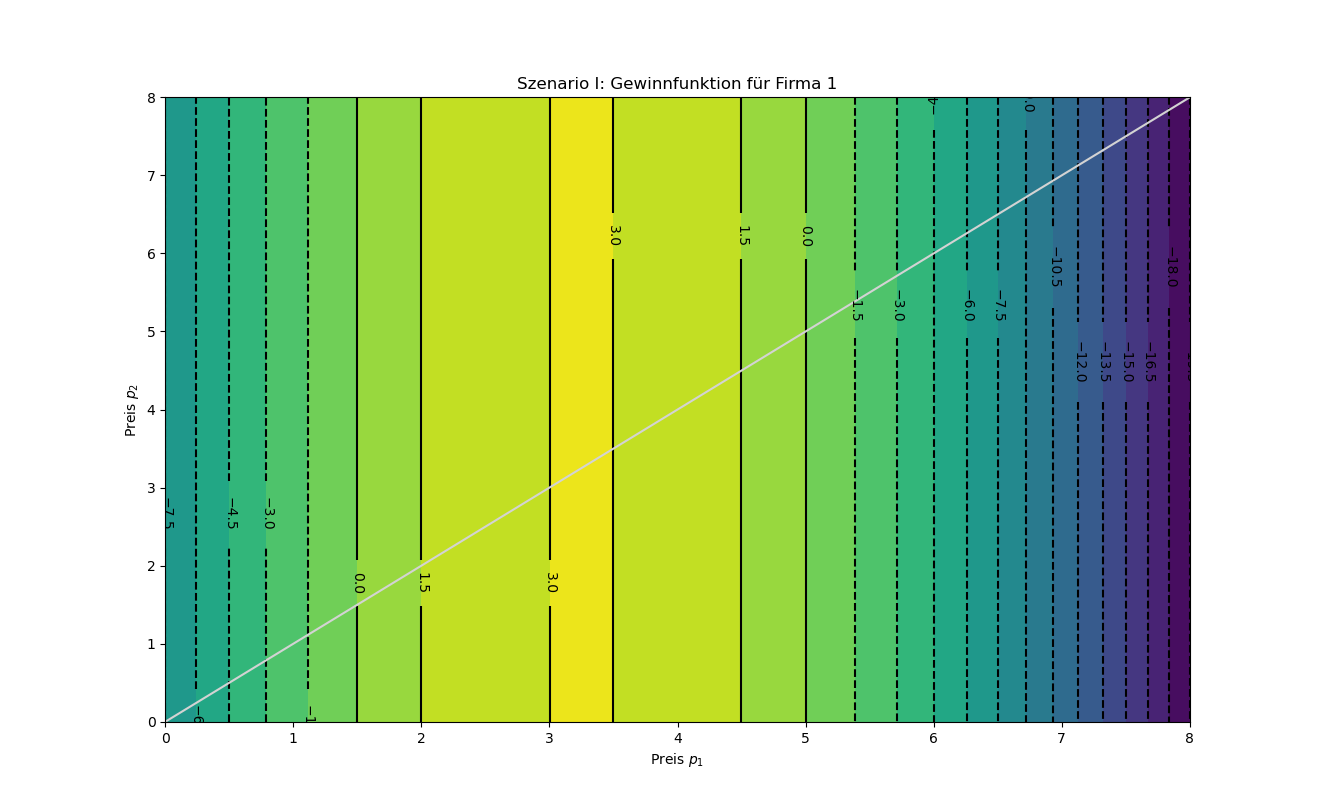
\includegraphics[width=0.8\textwidth]{nash1.png}
\end{center}
\caption{Gewinnfunktion aus Sicht des Unternehmens~1}
\label{fig:Grafik}
\end{figure}

\begin{itemize}
\item Ermitteln Sie den optimalen (maximalen) Gewinn, den beide Unternehmen jeweils erzielen können.
\item Ermitteln Sie die Anzahl der vorgenommenen Käufe gemäß Marktanalyse zu diesen Preisen.
\item Ermitteln Sie den dazu notwendigen optimalen Preis ($p_1=p_2=p$).
\item Zeichnen Sie den Punkt in die Grafik ein.
\end{itemize}


\section{Hintergrund}
Die Aufgabe beschreibt ein Maximierungsproblem und ist eine Warm-Up--Übung für das Szenario II, bei dem es dann um ein sogenanntes  \emph{Nash--Gleichgewicht} gehen wird.
Bei einem \emph{Nash--Gleichgewicht} wenden beide Parteien eine optimale Strategie an, die unabhängig von der gewählten Strategie der anderen Partei ist.

Beide Parteien wählen simultan ihre Strategie und bleiben auch dabei. Das \emph{Nash--Gleichgewicht} gehört zum Bereich der \emph{Spieltheorie}.

Entdecker dieses besonderen Gleichgewichts ist John Nash\footnote{(John Forbes Nash Jr., \textborn 13. Juni 1928 in Bluefield, West Virginia; \textdied 23. Mai 2015 nahe Monroe Township, New Jersey)}, Hauptfigur des Filmes \emph{A Beautiful Mind}. In der Volkswirtschaftslehre gehört diese Aufgabenstellung in den Bereich der Mikroökonomie/Spieltheorie.

\section{Abgabe und Zeitrahmen}
Die Aufgabe ist \emph{optional} und kann während des Dezembers/Jahreswende bearbeitet werden.
Interessant ist, wie genau die geforderten Werte bestimmt werden können.

\ifloesung
\newpage
\section{Musterlösung}

\newpage
\mylisting[label=musterloesung1]{Musterlösung}{pirate.c}{c}


\fi
\end{document}